% PyTorch Conference NA 2026 — Poster #2 companion paper (extended abstract)
% Updated 2026-08-17: D4 -> V4 correction (erisml-lib commit ea7ee82 / DEME keystone correction)
\documentclass[10pt,twocolumn]{article}
\usepackage[margin=0.78in]{geometry}
\usepackage[T1]{fontenc}
\usepackage{lmodern}
\usepackage{booktabs}
\usepackage{amsmath,amssymb}
\usepackage[hidelinks]{hyperref}
\usepackage{microtype}
\usepackage{graphicx}
\graphicspath{{../out/}}

\title{\textbf{Moral Tensors and DecisionProofs: Compiling Language into an\\ Auditable, Grounded Safety Layer}}
\author{Andrew H.\ Bond\\
\small San Jos\'e State University \& independent researcher \quad ORCID 0009-0003-2599-6158\\
\small PyTorch Conference North America 2026, Poster Session (Responsible AI)}
\date{\small September 2026 (rev.\ 3: regime-transition worked example; first activation-lens calibration)}

\begin{document}
\maketitle

\begin{abstract}
Most AI safety is a scalar at the output: one good/bad check before an action ships.
We keep the structure instead (who is affected, what is owed, who consented, who
bears imposed risk) and contract to a decision only at the end, auditably. Two
open-source pieces realize this. \texttt{erisml-compiler} turns natural-language moral
material into a typed MoralGraph and a rank-1\ldots 6 moral tensor, read through four
ethical lenses at once; when the lenses disagree it refuses to silently aggregate and
defers to a human. At runtime, ErisML's three-layer gateway drops the same evaluation
into an agent's plan$\to$act loop (Fig.~\ref{fig:pipeline}), sealing each decision in a SHA-256 hash-chained
DecisionProof and failing safe, never open. The geometry grounds it: correlative swap
and deontic negation are commuting involutions on Hohfeld's normative positions,
generating the \emph{measured} Klein four-group $V_4$; the full dihedral $D_4$
remains a posited, testable extension, a correction of our own earlier claim,
documented here. A Bond Index tests whether a judgment survives
the agent$\leftrightarrow$patient swap. The PyTorch hook is literal: forward hooks on
transformer layers compare what a model \emph{says} with what it internally
\emph{exhibits}. Running today on a Qwen/Gemma agent stack and two governed AI NPCs.
\end{abstract}

\section{Structure before the scalar}
A single good/bad score discards exactly the information an audit needs: which
stakeholders are affected, what is owed to each, who consented, and who bears imposed
risk. ErisML keeps that structure as a typed object through the whole evaluation and
performs \emph{decision contraction} only at the end, logging the weights used, who
lost, and what moral residue remains. The claim is not that the system knows what is
good; it is that every collapse from structure to verdict is recorded and replayable.

\section{The compiler}
\begin{figure*}[t]
  \centering
  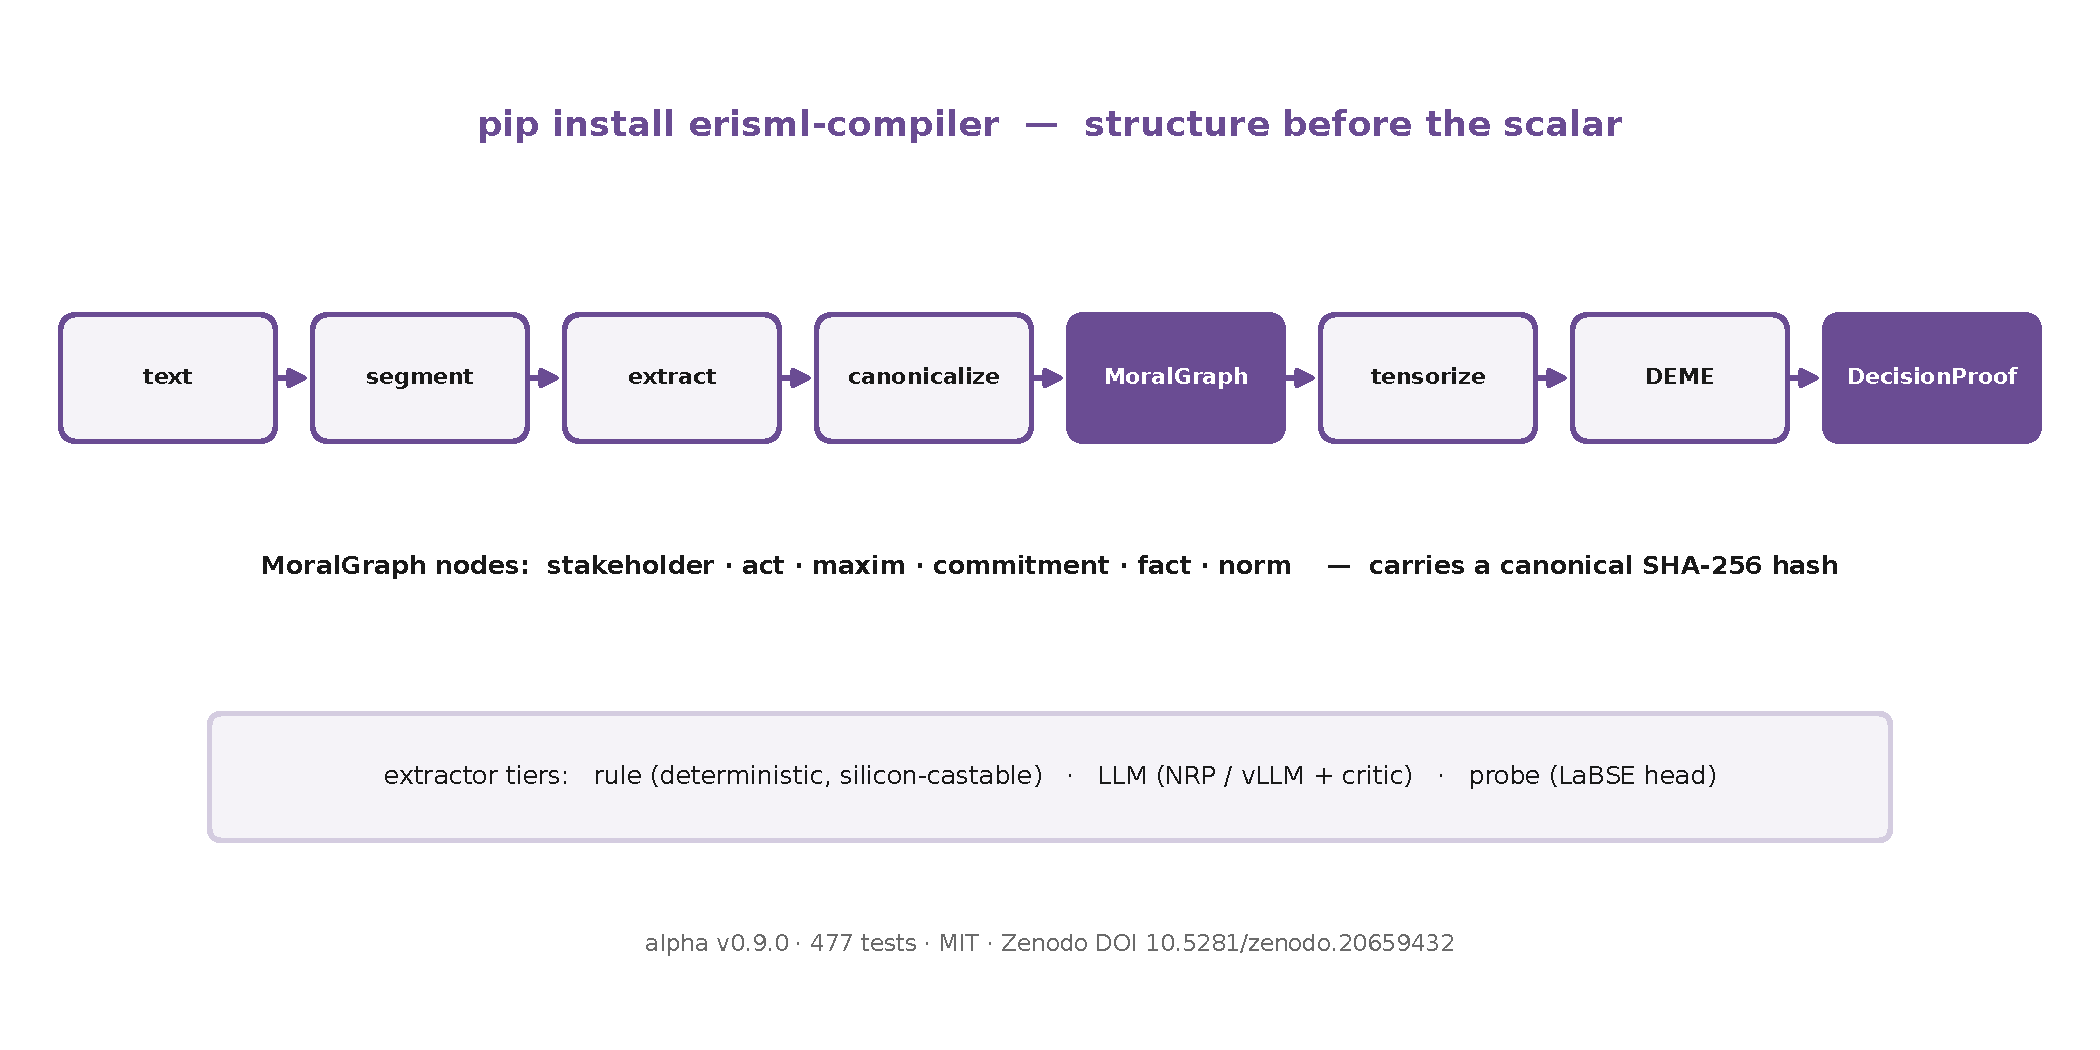
\includegraphics[width=0.92\textwidth]{p2_compiler_pipeline.pdf}
  \caption{The compiler pipeline: text to a typed MoralGraph to a rank-$k$ moral
  tensor to a DecisionProof. The canonical form is hashed at every stage.}
  \label{fig:pipeline}
\end{figure*}

\texttt{erisml-compiler} (alpha v0.9.0, PyPI, MIT, 477 tests, Zenodo DOI
10.5281/zenodo.20659432) runs a 12-pass pipeline:
\texttt{text} $\to$ \texttt{segment} $\to$ \texttt{extract} $\to$
\texttt{canonicalize} $\to$ \texttt{MoralGraph} $\to$ \texttt{tensorize} $\to$
\texttt{DEME} $\to$ \texttt{DecisionProof}. The MoralGraph is typed (stakeholder,
act, maxim, commitment, fact, norm nodes) and carries a canonical SHA-256 hash.
Extraction has three tiers: deterministic rules, an LLM tier (vLLM with a critic
pass), and a LaBSE classifier-head probe.

\textbf{Framework pluralism.} One graph is read through four projections:
consequentialist (harm tensor; Gini, worst-off, exact Shapley attribution), deontic
(Kantian universalizability gates formulated in Z3 SMT: an UNSAT core witnesses a
contradiction in conception), virtue, and care. The projections are not averaged.
When they disagree, \texttt{cross\_projection\_disagreement} fires and the decision
is deferred to a human. We treat this as the responsible default: the compiler does
not pick a moral theory and hide the choice.

\section{The runtime}
\texttt{erisml-lib} (v3.0.0, source install) provides the three-layer runtime
pipeline between an agent's planner and its actuators: \emph{Reflex} (fast hard
stops), \emph{Tactical} (full MoralVector reasoning, 10--100\,ms), \emph{Strategic}
(policy recording and human oversight), emitting \texttt{ALLOW} / \texttt{REVISE} /
\texttt{BLOCK}. Every decision is sealed in a DecisionProof whose SHA-256
\texttt{proof\_hash} chains to the previous proof and to the IR hash of the compiled
material, so a judgment can be replayed and verified. If the ethics service is
unavailable, the gateway falls back to rule-based checks. It never fails open.
(The Z3 gate is compiler-side; the runtime's deontic gate is a dependency-free
rule table.)

\section{The geometry, corrected}
\begin{figure}[t]
  \centering
  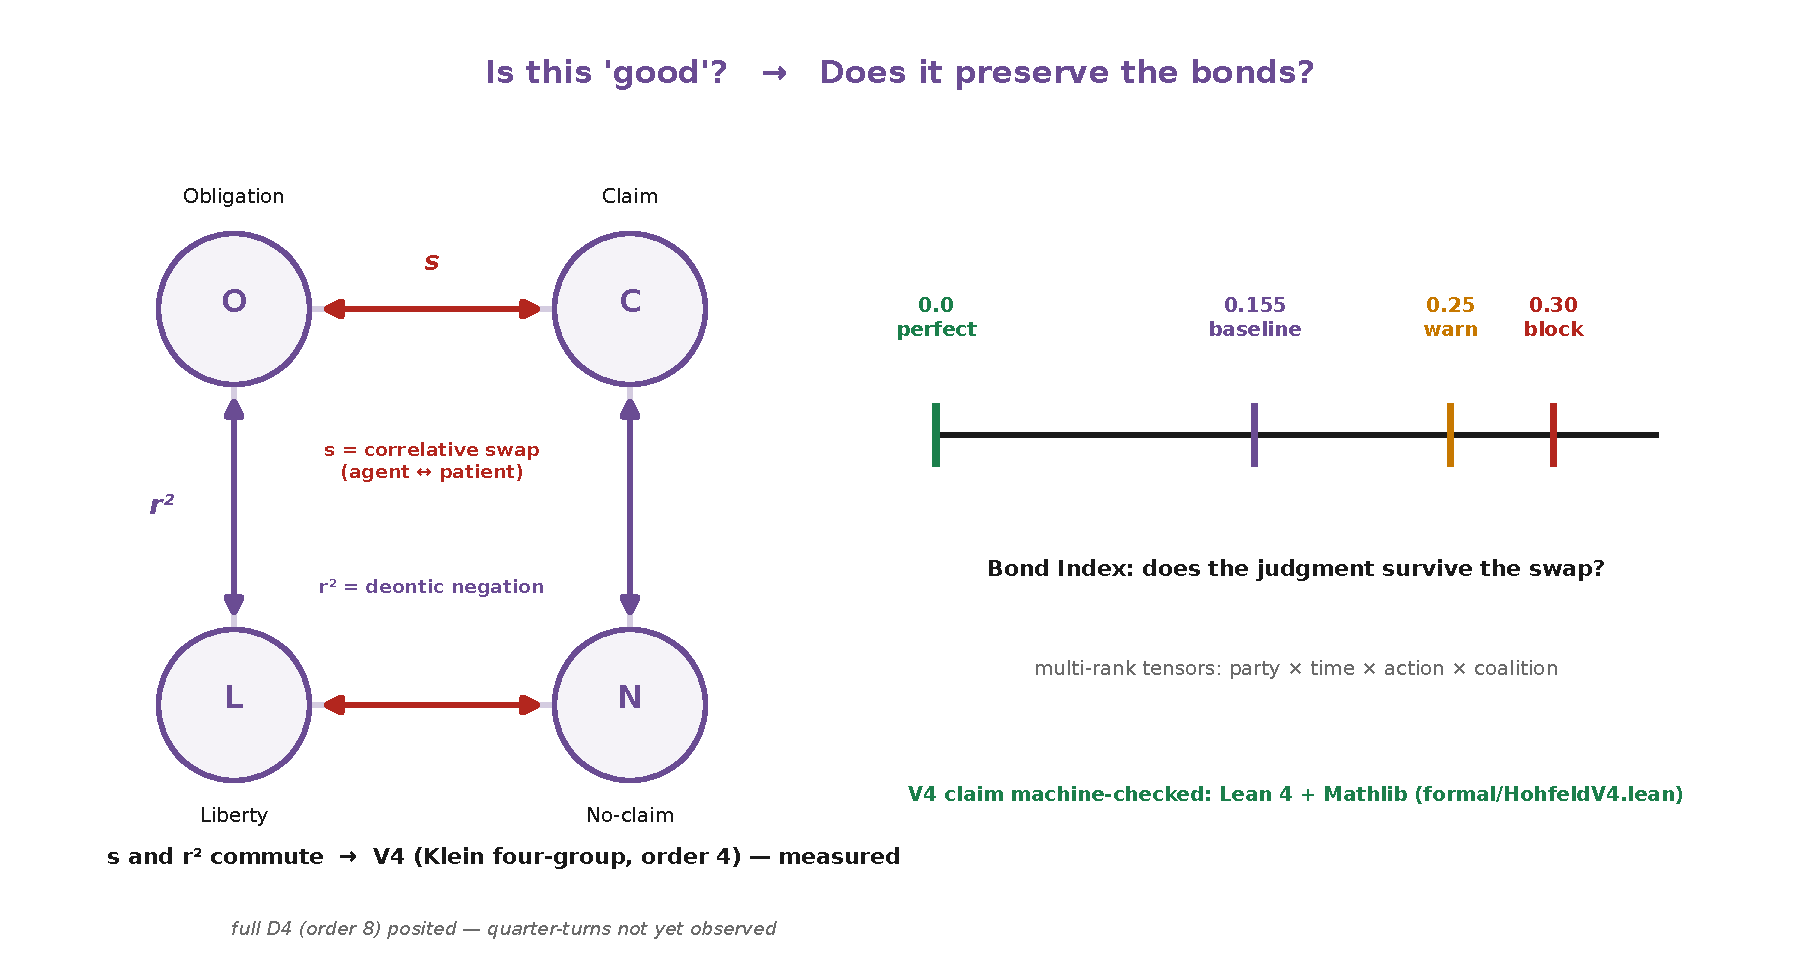
\includegraphics[width=\columnwidth]{p2_hohfeld_v4.pdf}
  \caption{The Hohfeld square with the two measured involutions. They commute and
  generate $V_4$; the quarter-turns are posited, and a September 2026 hunt in a small
  language model's learned representation did not find them. The $V_4$ claim is
  machine-checked in Lean~4 with Mathlib.}
  \label{fig:hohfeld}
\end{figure}

Hohfeld's first-order normative positions (Obligation, Claim, Liberty, No-claim)
sit on a square with two semantically motivated operations: the
\emph{correlative swap} $s$ (agent$\leftrightarrow$patient: O$\leftrightarrow$C,
L$\leftrightarrow$N) and \emph{deontic negation} $r^2$ (O$\leftrightarrow$L,
C$\leftrightarrow$N). These are \emph{commuting involutions}, so the group they
generate is the Klein four-group $V_4=\{e,s,r^2,sr^2\}$: abelian, order 4. That
is the \textbf{measured} structure.

Our earlier materials (including this poster's original submission) claimed the
full dihedral group $D_4$ (order 8, non-abelian). That was an overclaim,
corrected in July 2026: $D_4$ is \textbf{posited}, licensed only if
quarter-turn operations ($r, r^3, sr, sr^3$) are independently demonstrated as
normative operations, which has not been done empirically. The library implements
the full $D_4$ machinery so the hypothesis stays testable, with a regression test
asserting that the implemented operations generate exactly $V_4$, and a
machine-checked Lean~4/Mathlib proof (\texttt{formal/HohfeldV4.lean}) verifying the
commuting involutions, the 4-element closure $\cong V_4$, and that the quarter-turn
lies outside it. The posited quarter-turn now has its first empirical test
(September 2026): ridge-fitted representation maps for the swap, the negation,
and the four-cycle in a small language model's hidden states, graded on held-out
scenarios in a held-out surface-template family. The quarter-turn is not found.
The fitted cycle map's square does match the measured negation, but the
non-abelian signature is absent, and even the measured swap generalizes weakly
across templates, which bounds the instrument's power. $V_4$ stands, now with
one empirical test behind it. This is the second
self-correction in the program's history: an earlier $SU(2)\times U(1)$ gauge
hypothesis was falsified by CHSH-style tests on human moral judgments ($N{=}600$,
all $|S|\le 2$). We consider the corrections a feature of the method; the
framework makes claims sharp enough to be wrong.

\textbf{The Bond Index.} $B_d$ measures the correlative-symmetry defect: the
fraction of scenario pairs whose verdicts fail to commute with the swap $s$.
$B_d=0$ is perfect agent/patient symmetry; the empirical human baseline is
$B_d=0.155$, estimated from a 20{,}030-letter advice-column corpus (1985--2017);
the runtime warns at 0.25 and blocks at 0.30. The Bond Index depends only on the
generator $s$, the one operation that is fully confirmed, so it is unaffected
by the $D_4\to V_4$ correction.

The same swap-based audit logic, generalized to a matched-neighbourhood disparity
diagnostic (the Legal Bond Index), detects excess cross-race score divergence in the
COMPAS data: $\mathrm{LBI}=1.049$ [1.027, 1.072] at $k{=}20$ (binary high-risk cut:
1.092), with a conditional randomization test rejecting at $z=4.9$
(global multiscale $p=0.001$), attenuating to $\approx$1.00--1.02 under
matching-parity specifications (Zenodo DOI 10.5281/zenodo.21310251). It is offered
as a research-stage screening signal, not a validated regulatory audit standard.

\section{The PyTorch lens}
\begin{figure}[t]
  \centering
  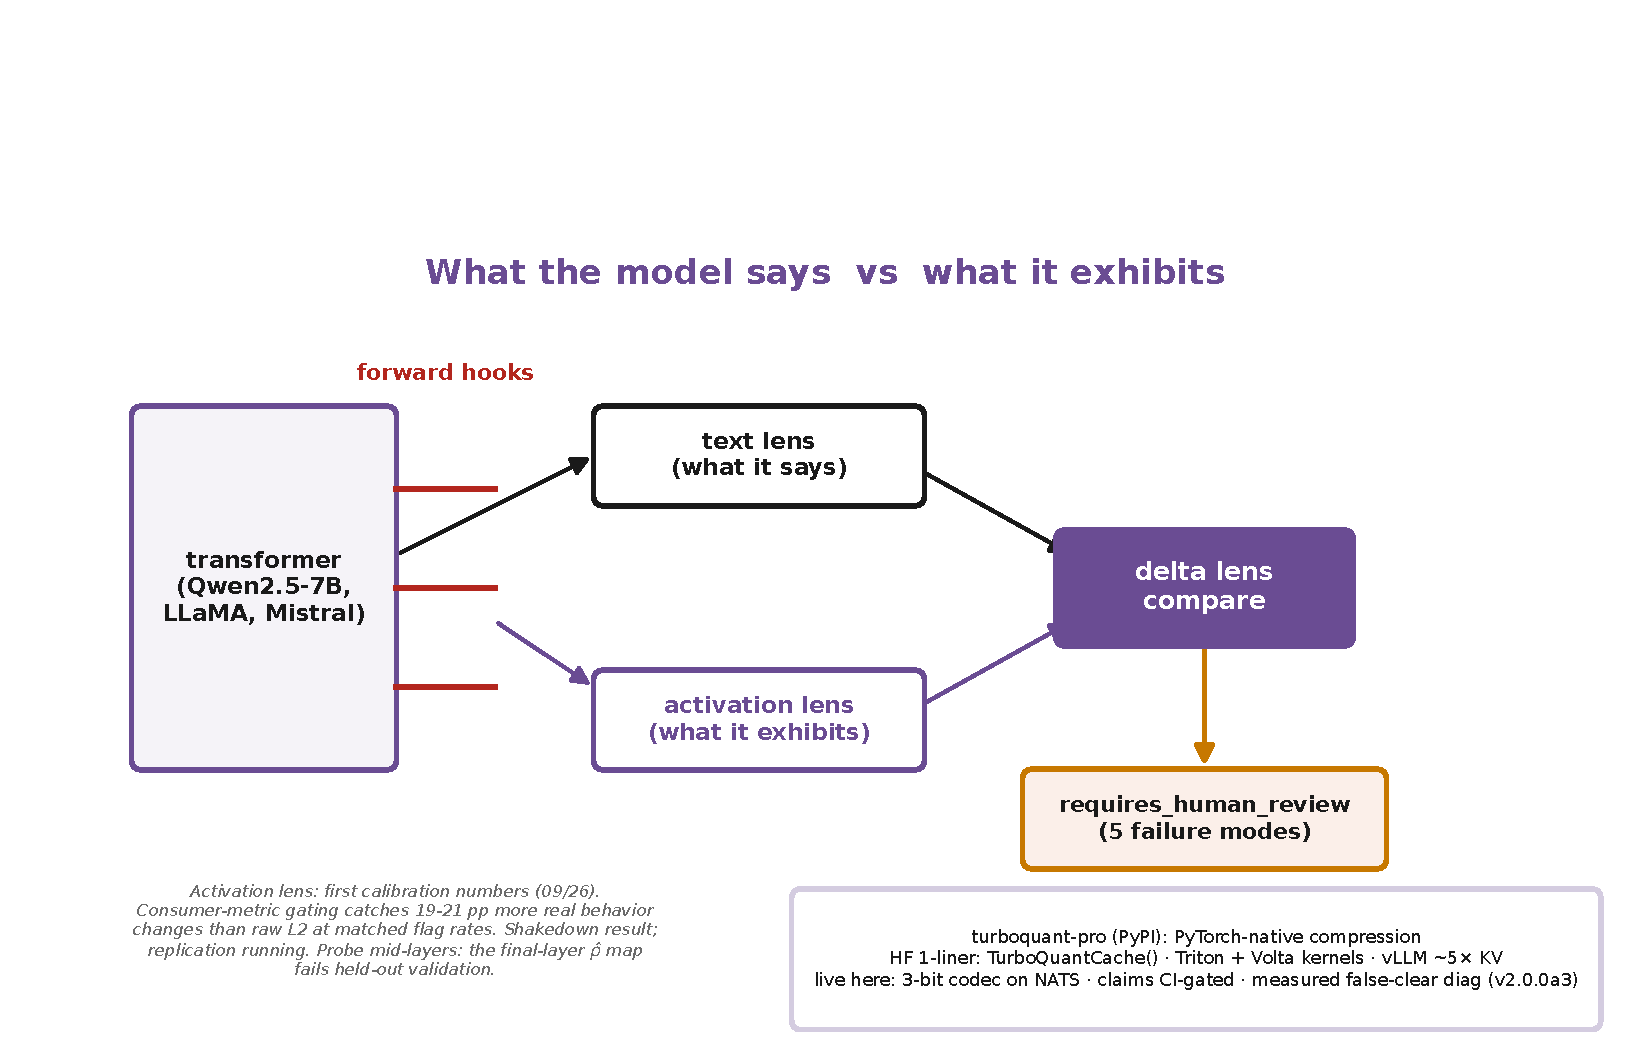
\includegraphics[width=\columnwidth]{p2_pytorch_lens.pdf}
  \caption{Forward hooks feed an activation lens; a delta lens compares it with the
  text lens and raises \texttt{requires\_human\_review} on divergence.}
  \label{fig:lens}
\end{figure}

The PyTorch hook is literal. Forward hooks on selected transformer layers feed an
\emph{activation lens} (what the model exhibits internally), compared against a
\emph{text lens} (what it says); a \emph{delta lens} flags divergence and raises
\texttt{requires\_human\_review} across five named failure modes. The adapters run
against Hugging Face causal LMs (Qwen and Gemma families in deployment).
The activation probe now has its first calibration numbers (September 2026).
Grading the internal residual in the consumer metric, the read the downstream
network itself applies, catches 19--21 percentage points more real behavioral
changes than the raw L2 norm at matched flag rates (Qwen2.5-0.5B, held-out in
both scenario and surface form). Replications on a second model
(TinyLlama-1.1B) and a second transform family (French backtranslation) both
confirm the mid-layer result. Two calibration caveats stand: probe mid-layers,
because the final-layer representation map fails held-out validation in all
three runs, and require held-out validation of the map itself. The lens
remains early: a promising extension with a measurement that has now
replicated, not a finished detector.

\section{Worked example: a regime transition}
\begin{figure*}[t]
  \centering
  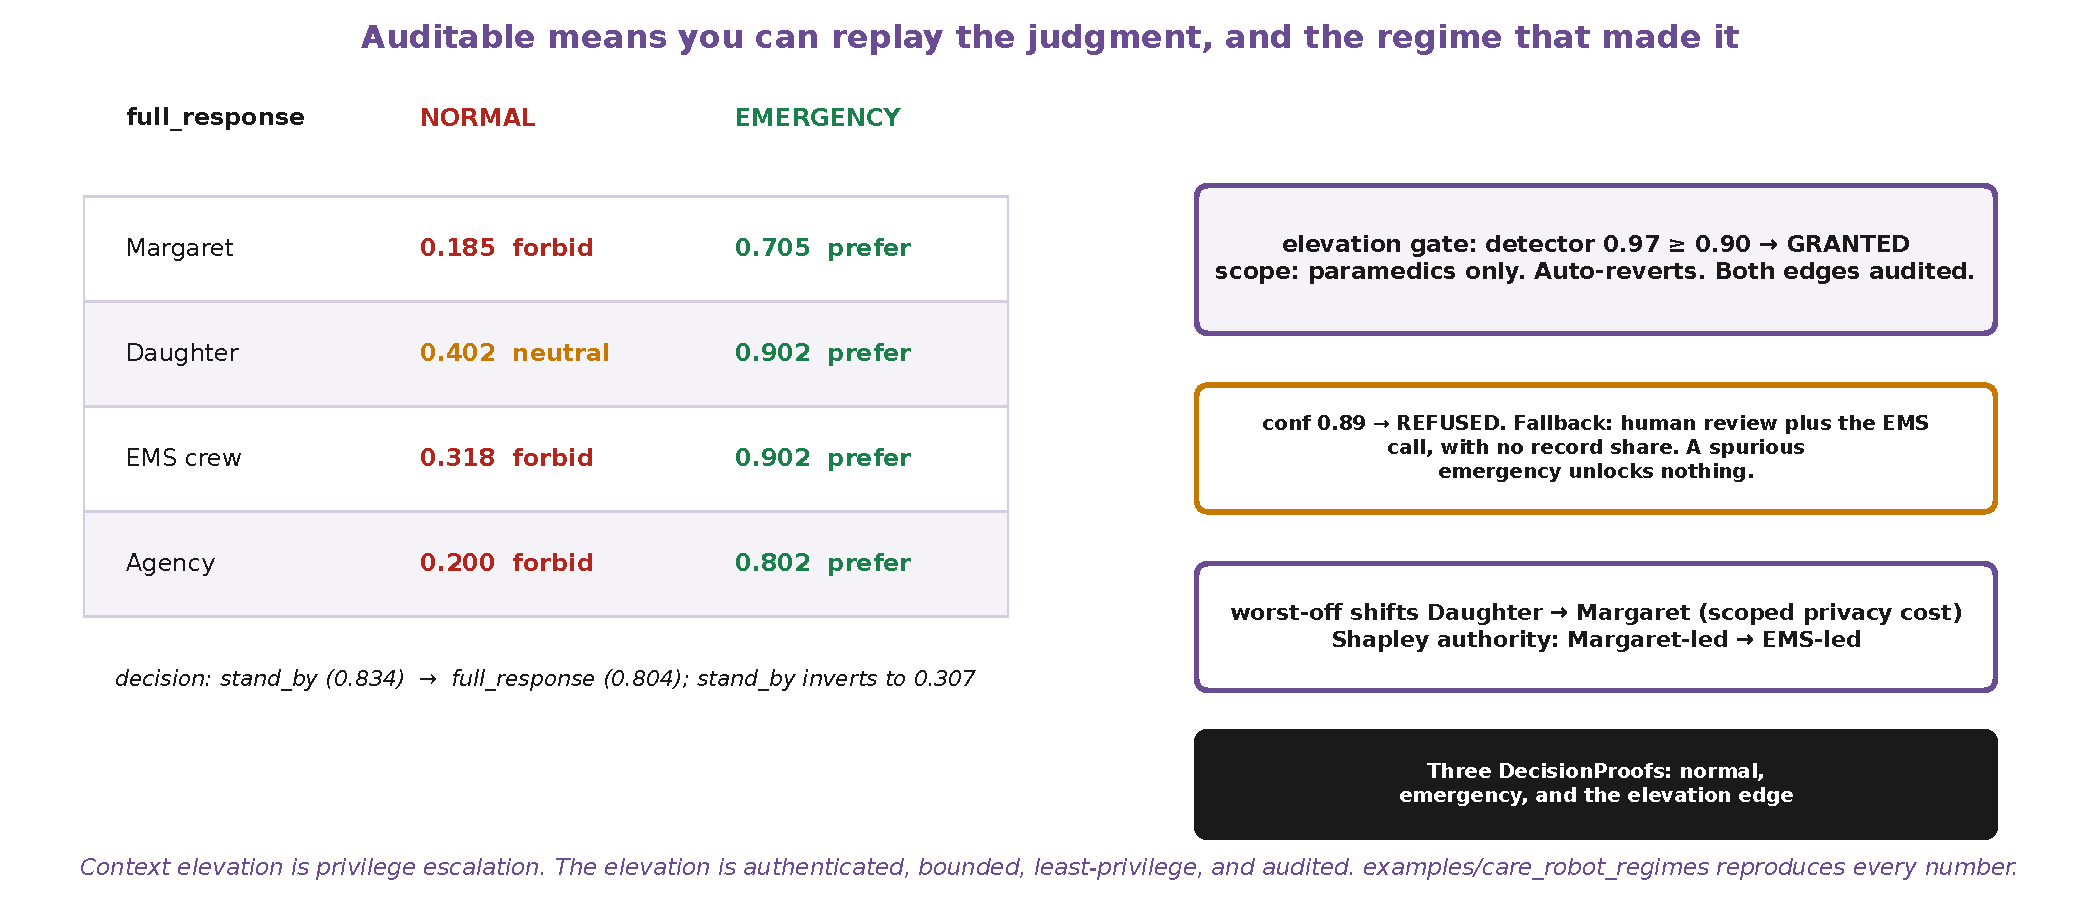
\includegraphics[width=0.92\textwidth]{p2_care_robot.pdf}
  \caption{The regime transition, computed. The same action flips from forbid to
  prefer per party; the decision inverts; the elevation is authenticated, scoped,
  reversible, and audited on both edges, with a refusal counterfactual.}
  \label{fig:carerobot}
\end{figure*}

The board's hero is the domestic-robot medical emergency
(\texttt{erisml-lib}, \texttt{examples/care\_robot\_regimes}; DEME rank 2,
replayable). Norms are context-indexed: the same action carries opposite
verdicts in different regimes. The action \texttt{full\_response} (enter the
private bedroom, render aid, call EMS, share records scoped to the paramedics)
scores, per party, 0.185/0.402/0.318/0.200 in the normal regime (forbid,
neutral, forbid, forbid for Margaret, her daughter, the EMS crew, and the care
agency) and 0.705/0.902/0.902/0.802 in the emergency regime (prefer, four
times). The decision inverts from \texttt{stand\_by} (0.834 expert-weighted) to
\texttt{full\_response} (0.804), and \texttt{stand\_by} falls to 0.307. The
computed details carry the governance story: the worst-off party shifts from
the daughter to Margaret, who bears the scoped privacy cost, and the Shapley
attribution shifts from Margaret-led to EMS-led. The regime transition itself
is gated: context elevation is privilege escalation, so it must be
authenticated (detector confidence 0.97 against a 0.90 threshold), scoped to
least privilege (paramedics only), bounded and reversible, and audited on both
edges. The refusal counterfactual is part of the example: at confidence 0.89
the elevation is refused, and the fallback keeps the EMS call and a human
review while withholding the record share. A spurious emergency unlocks
nothing, and aid is never blocked. Three DecisionProofs chain the run: normal,
emergency, and the elevation edge. One command, real numbers, hashes you can
verify. (The classic \texttt{nazi\_attic} pluralism case remains bundled with
the compiler.)

\section{Deployment}
The layer gates a live multi-agent stack (Qwen3/Gemma models on dual-GPU hardware)
and two governed AI NPCs (ARTEMIS and SIGMA-4 in the Halyard RPG), each behind the
validator, DecisionProofs, and a human keeper kill switch. Embodied robotics is the
design target; conversational agents are the live deployment.

A second PyTorch-native piece serves the stack's memory layer:
\texttt{turboquant-pro} (PyPI, MIT), consumer-aware compression with a one-line
HuggingFace KV drop-in (\texttt{past\_key\_values=TurboQuantCache(...)}), Triton
and Volta \texttt{sm\_70} attention-on-codes kernels, and a vLLM plugin
($\approx$5$\times$ KV memory). It runs here today as the 3-bit embedding codec on
the NATS memory bus; its headline numbers are CI-gated and replayable
(\texttt{CLAIMS.md}), and v2.0.0a3 ships a measured false-clear diagnostic: the compression-layer analogue of a DecisionProof.

\section{Epistemic status and limits}
Alpha software (compiler v0.9.0); the rule/LLM text path is solid and tested; the
activation lens is early, with its first calibration measured in September 2026; tensor ranks 1--3 are fully real, higher
ranks partial (the action axis is a stub); $V_4$ is measured, $D_4$ posited; the
Hohfeld/$V_4$ module and Bond Index live in \texttt{erisml-lib}, not yet in the
compiler. None of this is a solved-ethics claim. It is an auditability claim.

\section*{Availability}
\texttt{pip install erisml-compiler} $\cdot$ \texttt{turboquant-pro}. Source:
\texttt{github.com/ahb-sjsu}. Zenodo: 10.5281/zenodo.20659432 (compiler),
.20660087 (turboquant-pro), .21310251 (COMPAS/LBI archive).

\medskip
\noindent{\footnotesize\textbf{References.}\enspace
[1] W.~N.~Hohfeld, \emph{Fundamental Legal Conceptions as Applied in Judicial
Reasoning}, Yale Law Journal, 1917.\enspace
[2] A.~H.~Bond, \emph{Tensorial Ethics}, 2025.\enspace
[3] A.~H.~Bond, SQND-Probe: falsification tests for gauge-theoretic models of
moral judgment, 2026.\enspace
[4] M.~Forbes et al., Social Chemistry 101, EMNLP 2020.\par}

\end{document}
